% Options for packages loaded elsewhere
\PassOptionsToPackage{unicode}{hyperref}
\PassOptionsToPackage{hyphens}{url}
\PassOptionsToPackage{dvipsnames,svgnames,x11names}{xcolor}
%
\documentclass[
  letterpaper,
  DIV=11,
  numbers=noendperiod]{scrartcl}

\usepackage{amsmath,amssymb}
\usepackage{iftex}
\ifPDFTeX
  \usepackage[T1]{fontenc}
  \usepackage[utf8]{inputenc}
  \usepackage{textcomp} % provide euro and other symbols
\else % if luatex or xetex
  \usepackage{unicode-math}
  \defaultfontfeatures{Scale=MatchLowercase}
  \defaultfontfeatures[\rmfamily]{Ligatures=TeX,Scale=1}
\fi
\usepackage[sfmath]{kpfonts}
\ifPDFTeX\else  
    % xetex/luatex font selection
\fi
% Use upquote if available, for straight quotes in verbatim environments
\IfFileExists{upquote.sty}{\usepackage{upquote}}{}
\IfFileExists{microtype.sty}{% use microtype if available
  \usepackage[]{microtype}
  \UseMicrotypeSet[protrusion]{basicmath} % disable protrusion for tt fonts
}{}
\makeatletter
\@ifundefined{KOMAClassName}{% if non-KOMA class
  \IfFileExists{parskip.sty}{%
    \usepackage{parskip}
  }{% else
    \setlength{\parindent}{0pt}
    \setlength{\parskip}{6pt plus 2pt minus 1pt}}
}{% if KOMA class
  \KOMAoptions{parskip=half}}
\makeatother
\usepackage{xcolor}
\setlength{\emergencystretch}{3em} % prevent overfull lines
\setcounter{secnumdepth}{5}
% Make \paragraph and \subparagraph free-standing
\makeatletter
\ifx\paragraph\undefined\else
  \let\oldparagraph\paragraph
  \renewcommand{\paragraph}{
    \@ifstar
      \xxxParagraphStar
      \xxxParagraphNoStar
  }
  \newcommand{\xxxParagraphStar}[1]{\oldparagraph*{#1}\mbox{}}
  \newcommand{\xxxParagraphNoStar}[1]{\oldparagraph{#1}\mbox{}}
\fi
\ifx\subparagraph\undefined\else
  \let\oldsubparagraph\subparagraph
  \renewcommand{\subparagraph}{
    \@ifstar
      \xxxSubParagraphStar
      \xxxSubParagraphNoStar
  }
  \newcommand{\xxxSubParagraphStar}[1]{\oldsubparagraph*{#1}\mbox{}}
  \newcommand{\xxxSubParagraphNoStar}[1]{\oldsubparagraph{#1}\mbox{}}
\fi
\makeatother


\providecommand{\tightlist}{%
  \setlength{\itemsep}{0pt}\setlength{\parskip}{0pt}}\usepackage{longtable,booktabs,array}
\usepackage{calc} % for calculating minipage widths
% Correct order of tables after \paragraph or \subparagraph
\usepackage{etoolbox}
\makeatletter
\patchcmd\longtable{\par}{\if@noskipsec\mbox{}\fi\par}{}{}
\makeatother
% Allow footnotes in longtable head/foot
\IfFileExists{footnotehyper.sty}{\usepackage{footnotehyper}}{\usepackage{footnote}}
\makesavenoteenv{longtable}
\usepackage{graphicx}
\makeatletter
\newsavebox\pandoc@box
\newcommand*\pandocbounded[1]{% scales image to fit in text height/width
  \sbox\pandoc@box{#1}%
  \Gscale@div\@tempa{\textheight}{\dimexpr\ht\pandoc@box+\dp\pandoc@box\relax}%
  \Gscale@div\@tempb{\linewidth}{\wd\pandoc@box}%
  \ifdim\@tempb\p@<\@tempa\p@\let\@tempa\@tempb\fi% select the smaller of both
  \ifdim\@tempa\p@<\p@\scalebox{\@tempa}{\usebox\pandoc@box}%
  \else\usebox{\pandoc@box}%
  \fi%
}
% Set default figure placement to htbp
\def\fps@figure{htbp}
\makeatother
% definitions for citeproc citations
\NewDocumentCommand\citeproctext{}{}
\NewDocumentCommand\citeproc{mm}{%
  \begingroup\def\citeproctext{#2}\cite{#1}\endgroup}
\makeatletter
 % allow citations to break across lines
 \let\@cite@ofmt\@firstofone
 % avoid brackets around text for \cite:
 \def\@biblabel#1{}
 \def\@cite#1#2{{#1\if@tempswa , #2\fi}}
\makeatother
\newlength{\cslhangindent}
\setlength{\cslhangindent}{1.5em}
\newlength{\csllabelwidth}
\setlength{\csllabelwidth}{3em}
\newenvironment{CSLReferences}[2] % #1 hanging-indent, #2 entry-spacing
 {\begin{list}{}{%
  \setlength{\itemindent}{0pt}
  \setlength{\leftmargin}{0pt}
  \setlength{\parsep}{0pt}
  % turn on hanging indent if param 1 is 1
  \ifodd #1
   \setlength{\leftmargin}{\cslhangindent}
   \setlength{\itemindent}{-1\cslhangindent}
  \fi
  % set entry spacing
  \setlength{\itemsep}{#2\baselineskip}}}
 {\end{list}}
\usepackage{calc}
\newcommand{\CSLBlock}[1]{\hfill\break\parbox[t]{\linewidth}{\strut\ignorespaces#1\strut}}
\newcommand{\CSLLeftMargin}[1]{\parbox[t]{\csllabelwidth}{\strut#1\strut}}
\newcommand{\CSLRightInline}[1]{\parbox[t]{\linewidth - \csllabelwidth}{\strut#1\strut}}
\newcommand{\CSLIndent}[1]{\hspace{\cslhangindent}#1}

\KOMAoption{captions}{tableheading}
\makeatletter
\@ifpackageloaded{tcolorbox}{}{\usepackage[skins,breakable]{tcolorbox}}
\@ifpackageloaded{fontawesome5}{}{\usepackage{fontawesome5}}
\definecolor{quarto-callout-color}{HTML}{909090}
\definecolor{quarto-callout-note-color}{HTML}{0758E5}
\definecolor{quarto-callout-important-color}{HTML}{CC1914}
\definecolor{quarto-callout-warning-color}{HTML}{EB9113}
\definecolor{quarto-callout-tip-color}{HTML}{00A047}
\definecolor{quarto-callout-caution-color}{HTML}{FC5300}
\definecolor{quarto-callout-color-frame}{HTML}{acacac}
\definecolor{quarto-callout-note-color-frame}{HTML}{4582ec}
\definecolor{quarto-callout-important-color-frame}{HTML}{d9534f}
\definecolor{quarto-callout-warning-color-frame}{HTML}{f0ad4e}
\definecolor{quarto-callout-tip-color-frame}{HTML}{02b875}
\definecolor{quarto-callout-caution-color-frame}{HTML}{fd7e14}
\makeatother
\makeatletter
\@ifpackageloaded{caption}{}{\usepackage{caption}}
\AtBeginDocument{%
\ifdefined\contentsname
  \renewcommand*\contentsname{Table of contents}
\else
  \newcommand\contentsname{Table of contents}
\fi
\ifdefined\listfigurename
  \renewcommand*\listfigurename{List of Figures}
\else
  \newcommand\listfigurename{List of Figures}
\fi
\ifdefined\listtablename
  \renewcommand*\listtablename{List of Tables}
\else
  \newcommand\listtablename{List of Tables}
\fi
\ifdefined\figurename
  \renewcommand*\figurename{図}
\else
  \newcommand\figurename{図}
\fi
\ifdefined\tablename
  \renewcommand*\tablename{Table}
\else
  \newcommand\tablename{Table}
\fi
}
\@ifpackageloaded{float}{}{\usepackage{float}}
\floatstyle{ruled}
\@ifundefined{c@chapter}{\newfloat{codelisting}{h}{lop}}{\newfloat{codelisting}{h}{lop}[chapter]}
\floatname{codelisting}{Listing}
\newcommand*\listoflistings{\listof{codelisting}{List of Listings}}
\makeatother
\makeatletter
\makeatother
\makeatletter
\@ifpackageloaded{caption}{}{\usepackage{caption}}
\@ifpackageloaded{subcaption}{}{\usepackage{subcaption}}
\makeatother

\usepackage{bookmark}

\IfFileExists{xurl.sty}{\usepackage{xurl}}{} % add URL line breaks if available
\urlstyle{same} % disable monospaced font for URLs
\hypersetup{
  pdftitle={法律家のための統計数理(1)確率論入門},
  pdfauthor={司馬博文},
  colorlinks=true,
  linkcolor={ParisGreen},
  filecolor={ParisGreen},
  citecolor={ParisGreen},
  urlcolor={ParisGreen},
  pdfcreator={LaTeX via pandoc}}


\title{法律家のための統計数理(1)確率論入門}
\usepackage{etoolbox}
\makeatletter
\providecommand{\subtitle}[1]{% add subtitle to \maketitle
  \apptocmd{\@title}{\par {\large #1 \par}}{}{}
}
\makeatother
\subtitle{教科書第1章第1節 (pp.~1-14)}
\author{司馬博文}
\date{11/22/2023}

\begin{document}
\maketitle
\begin{abstract}
教科書第1章第1節(pp.1-14)までの内容を,確率論の公理と数学の考え方を補足しながら,自分の言葉で導出しなおした.
\end{abstract}

\renewcommand*\contentsname{Table of contents}
{
\hypersetup{linkcolor=}
\setcounter{tocdepth}{3}
\tableofcontents
}

(\citeproc{ref-ux8349ux91ceux8015ux4e002016}{草野耕一, 2016})
の勉強会第1回の補足として,確率論の数学的枠組みを紹介する.

\begin{figure}[H]

{\centering 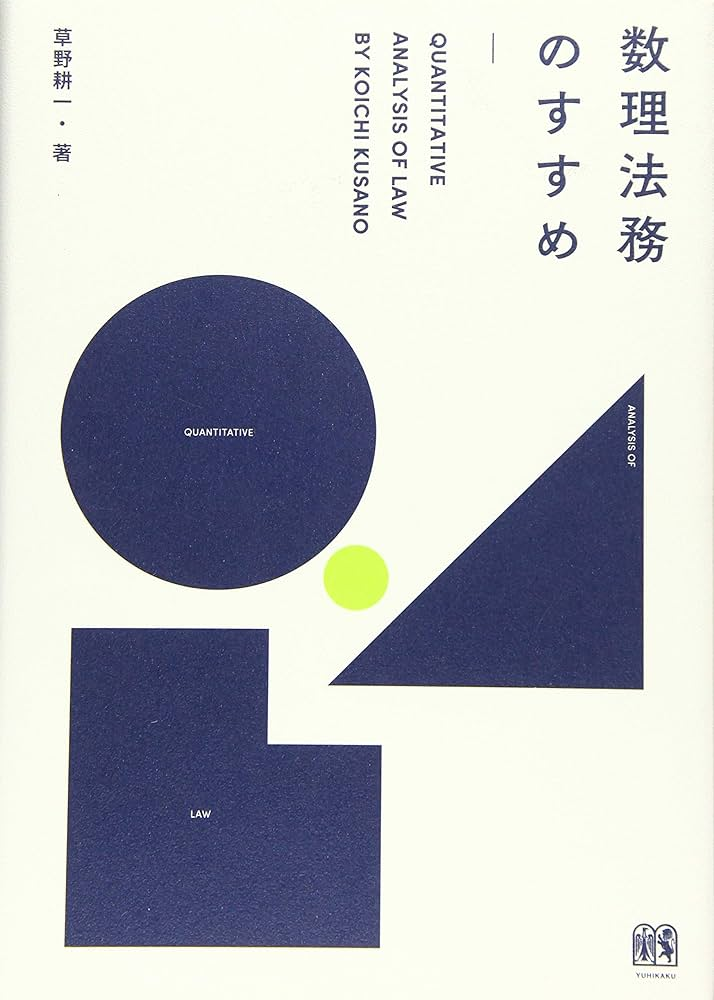
\includegraphics[width=1.04167in,height=\textheight,keepaspectratio]{草野耕一.jpg}

}

\caption{本勉強会の指定教科書}

\end{figure}%

参考書としては (\citeproc{ref-ux5927ux585a2020}{大塚淳, 2020})
もおすすめ.

シリーズトップページは\href{../../../static/Sessions.qmd\#sec-法律家のための統計数理}{こちら}.

\subsection{今回の内容}\label{ux4ecaux56deux306eux5185ux5bb9}

\subsubsection{本書の概観}\label{ux672cux66f8ux306eux6982ux89b3}

本書は「数理法務」=「法の数理分析」に関する発展的内容を扱った書籍で,内容は大きく次の1から3の3つからなる:

\begin{enumerate}
\def\labelenumi{\arabic{enumi}.}
\tightlist
\item
  法の行動分析:法律家がとるべき行動を数理を用いて分析する.
\item
  法の統計分析:事実の推定や因果関係の推定に統計手法を応用する.
\item
  法の財務分析:企業や金融に関わる法事象をファイナンス理論を用いて分析する.
\item
  法の経済分析:法を経済学的な観点から分析する(本書では扱われていない).
\end{enumerate}

第1回勉強会では第1章「行動分析(1)事実認定」を扱った.事実認定を,Bayes推論の枠組みで捉え直し,法律家として誤謬やバイアスに陥ってしまうことを避けるツールとして,確率論を導入しており,「法の数理分析は役に立つ」ことを端的に実感できる,導入として極めて鮮やかな章になっている.

\subsubsection{主観確率とBayes計算}\label{ux4e3bux89b3ux78baux7387ux3068bayesux8a08ux7b97}

まず,第1章は,事実認定の文脈で妥当な確率概念は「主観確率」であり,今後「確率」とはこの意味で用いることを注意喚起する内容から始まる.

主観確率と客観確率の詳細な定義は本書を参照願いたいが,一言で言えば,後者は「人間に不可知な真の値」というものの存在を前提とするのに対し,前者はそれを仮定しない.

従って,主観確率の考え方は,より多くのものに「確率」を導入することを可能にし,より柔軟な議論が可能であるが,その分数理的な困難も増し,真に発展が進んだと言えるのは,計算機が十分に爛熟した21世紀になってのことであると言える.この統計学分野を
\textbf{Bayes計算 (Bayesian Computation)} といい,筆者の研究分野である.

\begin{quote}
The development of computing algorithms especially suited for Bayesian
analysis in the 1990s together with the exponential growth of computing
resources enabled Bayesian nonparametrics to go beyond the simplest
problems and made it a universally applicable paradigm for inference.
(\citeproc{ref-Ghosal-vanderVaart17-NonparametricBayes}{Ghosal and
van~der~Vaart, 2017})
\end{quote}

\subsubsection{Bayes統計学とは?}\label{bayesux7d71ux8a08ux5b66ux3068ux306f}

大雑把に言って,客観確率に基づく統計手法を \textbf{頻度論的手法}
(frequentist methods),主観確率に対する統計手法を \textbf{Bayes手法}
(Bayesian
methods)という.一般に後者は前者を包含する(前者は後者の特別な場合\footnote{(\citeproc{ref-McElreath20-StatisticalRethinking}{McElreath,
  2020}) 1.3節.頻度論はさらに「仮想的な反復」(imaginary resampling of
  data)を想定する,という性質を除けば,不確実性が観測からくるもののみである特別な場合が頻度論であると捉えられる.})と考えられる.しかしこれは「確率の解釈」が違うのみであり,数学としては確率の定義は1つである.「確率の解釈」については,双方の立場の中でもそれぞれ複数の立場が乱立しており,ここでは立ち入らない.と言っても,この注記も教科書的なもので,実用上不便を生じる場面はほとんどないだろう.

\begin{quote}
不確実性を定量化するのに、ベイズ計算では必ず『確率』を使います。一般の人から見たら、統計で確率を使うのは当たり前と思うでしょうが、じつは他の統計手法ではそうでもなく、さまざまな解釈が生まれてしまう。\textbf{定量化にはすべて統一的に確率を使うベイズ計算は、非常にシンプルなので、最終的にすべての統計はベイズに行き着くしかないと思っています。}
\href{https://www.ism.ac.jp/ism_info_j/labo/project/162.html}{鎌谷研吾}
\end{quote}

\subsubsection{Bayes確率の基礎付けの試み\ldots\ldots!?}\label{bayesux78baux7387ux306eux57faux790eux4ed8ux3051ux306eux8a66ux307f}

法律家による事実認定の文脈においても,「真実はいつも1つだからそれを推定したい」と考えても,「不確実な中でも,判断を誤らないようにしたい」と考えても,どちらから議論しても良いことは納得いただけるだろう.ただ,一般の人の素朴な「確率」の理解は,Bayes流のものに近いと言われている.\footnote{(\citeproc{ref-McElreath20-StatisticalRethinking}{McElreath,
  2020}) 1.3節,(\citeproc{ref-Rubin84-ABC}{Rubin, 1984}).}

そのこともあり,本書で「主観確率の考え方を採用する」というのは,「確率の解釈の議論はここではしない」「主観的な確信度合いの意味で,現実から多少の乖離を許す」という程度の意味であろう.

しかし,本書の「主観確率」の議論は中途半端な取り扱いでは終わらず,興味深いことに,One
More Step 1-1 (pp.9-10)
にて,数理哲学者\href{https://en.wikipedia.org/wiki/Donald_A._Gillies}{Donald
A.
Gillies}による主観確率の測定による基礎付けの議論が紹介されていた.筆者は初耳の議論であり,己の議論の正統性・基礎付けに細心の注意を施す法律家の心が現れていると筆者は見た.

\subsection{【深掘り】確率の公理}\label{sec-2}

\subsubsection{「確率の公理」がなぜ重要なのか?}\label{ux78baux7387ux306eux516cux7406ux304cux306aux305cux91cdux8981ux306aux306eux304b}

本書1.1節では確率の性質が列挙されている.1.2節以降では,これらの性質が「確率の定義」として引用されるが,いまいちどれを指して「定義」と呼んでいるのか定かでない.

数学的な議論に慣れたあとはそれでも良いかも知れないが,\textbf{法学も初学の間は逐一根拠条文に戻ることが大切であるように,数学もはっきりと定義を列挙し,「それのみを根拠とすること」を徹底することが大事である}.

なお,数学では何を定義として採用するかに任意性がある場合が多いが,唯一やってはいけないことは「定義が曖昧な状態で進むこと」である.そこで,せっかくであるから,現代数学が定義する最も筋の良い定義を採用して,本書の内容を俯瞰することにする.

\begin{quote}
人は,確率論のもった政治的,社会的意義を忘れてはならない.理知を一切の尺度として「代数学の炉火によって倫理学及び政治学を照さん」(Condorcet)
という時代精神,神の啓示に代らんとする確率論,それはフランス革命の思想的基礎に連関することを見失ってはならないのである.(\citeproc{ref-ux5317ux5dddux654fux753749-ux7d71ux8a08ux5b66ux306eux8a8dux8b58}{北川敏男,
1949})
\end{quote}

現代数学において,確率を特徴付けるものは「代数的性質」であり,それは次の3つのみに集約される.\footnote{Wikipediaページ\href{https://ja.wikipedia.org/wiki/\%E7\%A2\%BA\%E7\%8E\%87\%E3\%81\%AE\%E5\%85\%AC\%E7\%90\%86}{確率の公理}も参照.}

\subsubsection{確率の公理}\label{sec-axiom}

\begin{tcolorbox}[enhanced jigsaw, toprule=.15mm, leftrule=.75mm, titlerule=0mm, bottomtitle=1mm, title={定義(確率) {[}@Kolmogorov1931{]}}, arc=.35mm, toptitle=1mm, colbacktitle=quarto-callout-tip-color!10!white, coltitle=black, rightrule=.15mm, colback=white, opacityback=0, colframe=quarto-callout-tip-color-frame, opacitybacktitle=0.6, left=2mm, breakable, bottomrule=.15mm]

集合 \(\Omega\) 上の確率とは,次の3条件を満たす関数
\(P:\mathcal{P}(\Omega)\to\mathbb{R}\) である:\footnotemark{}\\
\strut ~~~{[}P1{]} \(P(\Omega)=1\).\\
\strut ~~~{[}P2{]} \(A\cap B=\emptyset\) ならば,
\[P(A\sqcup B)=P(A)+P(B).\]\\
\strut ~~~{[}P3{]} 任意の事象 \(A\subset\Omega\) について,
\[0\le P(A).\]\footnotemark{}

ただし,

\begin{itemize}
\tightlist
\item
  \(P\) の定義域 \(\mathcal{P}(\Omega)\) は「\(\Omega\)
  の部分集合全体の集合」のことである.これを \(\Omega\)
  の\textbf{冪集合}という.
\item
  \(A\sqcup B\) とは, \(A\cap B=\emptyset\) が成り立つときの \(A,B\)
  の合併 \(A\cup B\) を,\(A\cap B=\emptyset\)
  を強調して書き分ける記法とする.
\end{itemize}

\end{tcolorbox}

\footnotetext{関数とは,入力と出力の集合 \(X,Y\)
の間に定まる対応であって,任意の入力 \(x\in X\) に対してただ一つの出力
\(y\in Y\) が対応するもののことをいう.この対応を \(f(x)=y\) と表す.}

\footnotetext{後ろの2条件{[}P2{]}, {[}P3{]} のみを満たす関数 \(P\)
は「測度」という.そのため,確率は測度でもある.数学用語では「確率分布」は「確率測度」ともいう(例えば\href{https://ja.wikipedia.org/wiki/\%E7\%A2\%BA\%E7\%8E\%87\%E6\%B8\%AC\%E5\%BA\%A6}{このwikipediaページ}).}

この公理から,我々が日常的な感覚から「確率に成り立っていて欲しい性質」が全て導ける,ということが現代数学の重要な発見である.性質を見ていく前に,「定義」として,主要な概念に親しみやすい名前を付ける.そのすべての過程において,上の{[}P1{]},
{[}P2{]},
{[}P3{]}以外を用いていないことを確認することは,数学入門の際には非常に大事な営みである.\footnote{{[}P1{]}
  などの P は Probability のつもりである.}

\begin{tcolorbox}[enhanced jigsaw, toprule=.15mm, leftrule=.75mm, titlerule=0mm, bottomtitle=1mm, title={確率論に関連する用語}, arc=.35mm, toptitle=1mm, colbacktitle=quarto-callout-tip-color!10!white, coltitle=black, rightrule=.15mm, colback=white, opacityback=0, colframe=quarto-callout-tip-color-frame, opacitybacktitle=0.6, left=2mm, breakable, bottomrule=.15mm]

全体集合 \(\Omega\) は所与のものとする.\footnotemark{}

\begin{enumerate}
\def\labelenumi{\arabic{enumi}.}
\tightlist
\item
  \textbf{事象} とは,部分集合 \(A\subset\Omega\) のことをいう.
\item
  事象 \(A\subset\Omega\)
  の補集合\[A^\complement=\Omega\setminus A=\overline{A}:=\left\{\omega\in\Omega\mid \omega\notin A\right\}\]を
  \(A\)
  の\textbf{余事象}という.左から順に,数学で一般によく使われる記号である.\footnotemark{}
\item
  2つの事象 \(A,B\subset\Omega\) が \textbf{排反}
  であるとは,集合として共通部分を持たないことをいう:
  \(A\cap B=\emptyset\).
\end{enumerate}

\end{tcolorbox}

\footnotetext{集合にも公理があり,現代数学は\href{https://ja.wikipedia.org/wiki/\%E5\%85\%AC\%E7\%90\%86\%E7\%9A\%84\%E9\%9B\%86\%E5\%90\%88\%E8\%AB\%96}{ZFC公理系}の下で展開される.が,ここでは深入りしない.}

\footnotetext{\(\lnot A\) という記法について,\(\lnot\)
は論理記号であるから,集合 \(A\) に用いることは好ましくない.}

この3性質から,本書第1.1節にいう「確率の推論法則」が全て導出できる.

\subsubsection{式(1.1) p.4の証明}\label{ux5f0f1.1-p.4ux306eux8a3cux660e}

\begin{tcolorbox}[enhanced jigsaw, toprule=.15mm, leftrule=.75mm, titlerule=0mm, bottomtitle=1mm, title={式(1.1) p.4}, arc=.35mm, toptitle=1mm, colbacktitle=quarto-callout-tip-color!10!white, coltitle=black, rightrule=.15mm, colback=white, opacityback=0, colframe=quarto-callout-tip-color-frame, opacitybacktitle=0.6, left=2mm, breakable, bottomrule=.15mm]

任意の事象 \(A\subset\Omega\)
について,\[0\le P(A)\le 1.\]\footnotemark{}

\end{tcolorbox}

\footnotetext{確率は必ず\(0\)から\(1\)の値を取る,ということを主張している命題である.初学者はこれが「示すべき内容」として提示されていることに戸惑いを覚えるだろうが,現代数学では「これが示せるような必要最小限の定義が見つかった」ことに価値を見出す.}

\begin{tcolorbox}[enhanced jigsaw, toprule=.15mm, leftrule=.75mm, titlerule=0mm, bottomtitle=1mm, title={式(1.2) p.5}, arc=.35mm, toptitle=1mm, colbacktitle=quarto-callout-tip-color!10!white, coltitle=black, rightrule=.15mm, colback=white, opacityback=0, colframe=quarto-callout-tip-color-frame, opacitybacktitle=0.6, left=2mm, breakable, bottomrule=.15mm]

任意の事象 \(A\subset\Omega\) について, \[
P(A)+P(A^\complement)=1.
\]

\end{tcolorbox}

\begin{tcolorbox}[enhanced jigsaw, toprule=.15mm, leftrule=.75mm, titlerule=0mm, bottomtitle=1mm, title={証明}, arc=.35mm, toptitle=1mm, colbacktitle=quarto-callout-note-color!10!white, coltitle=black, rightrule=.15mm, colback=white, opacityback=0, colframe=quarto-callout-note-color-frame, opacitybacktitle=0.6, left=2mm, breakable, bottomrule=.15mm]

\(0\le P(A)\)
は{[}P3{]}に他ならない.式(1.2)も{[}P2{]}から従う.\(A\subset\Omega\)
の補集合を \(A^\complement:=\Omega\setminus A\) で表すと,
\(P(A^\complement)\ge0\) も成り立つから, \[
\begin{align*}
P(A)&\le P(A)+P(A^\complement)\\
&=P(A\sqcup A^\complement)\\
&=P(\Omega)=1.
\end{align*}
\]

\end{tcolorbox}

\subsubsection{式(1.3) p.5の証明}\label{ux5f0f1.3-p.5ux306eux8a3cux660e}

\begin{tcolorbox}[enhanced jigsaw, toprule=.15mm, leftrule=.75mm, titlerule=0mm, bottomtitle=1mm, title={式(1.3) p.5}, arc=.35mm, toptitle=1mm, colbacktitle=quarto-callout-tip-color!10!white, coltitle=black, rightrule=.15mm, colback=white, opacityback=0, colframe=quarto-callout-tip-color-frame, opacitybacktitle=0.6, left=2mm, breakable, bottomrule=.15mm]

任意の \(n\ge1\) について, \(n\) 個の事象
\(A_1,\cdots,A_n\subset\Omega\) が互いに排反であるとき, \[
\begin{align*}
&P(A_1)+P(A_2)+\cdots+P(A_n)\\
&\qquad\qquad=P(A_1\sqcup A_2\sqcup\cdots\sqcup A_n).
\end{align*}
\]

\end{tcolorbox}

\begin{tcolorbox}[enhanced jigsaw, toprule=.15mm, leftrule=.75mm, titlerule=0mm, bottomtitle=1mm, title={証明}, arc=.35mm, toptitle=1mm, colbacktitle=quarto-callout-note-color!10!white, coltitle=black, rightrule=.15mm, colback=white, opacityback=0, colframe=quarto-callout-note-color-frame, opacitybacktitle=0.6, left=2mm, breakable, bottomrule=.15mm]

\(n\) に関する数学的帰納法による.

\end{tcolorbox}

\subsubsection{式(1.4) p.6の証明}\label{ux5f0f1.4-p.6ux306eux8a3cux660e}

\begin{tcolorbox}[enhanced jigsaw, toprule=.15mm, leftrule=.75mm, titlerule=0mm, bottomtitle=1mm, title={式(1.4) p.6}, arc=.35mm, toptitle=1mm, colbacktitle=quarto-callout-tip-color!10!white, coltitle=black, rightrule=.15mm, colback=white, opacityback=0, colframe=quarto-callout-tip-color-frame, opacitybacktitle=0.6, left=2mm, breakable, bottomrule=.15mm]

任意の事象 \(A,B\subset\Omega\) について, \[
P(A)+P(B)=P(A\cup B)+P(A\cap B).
\]

\end{tcolorbox}

{[}P2{]} の条件は,\(A_1,A_2\)
が排反である場合に限定しており,その制限が邪魔であった.ここで一般の加法公式を得ることになる.

\begin{tcolorbox}[enhanced jigsaw, toprule=.15mm, leftrule=.75mm, titlerule=0mm, bottomtitle=1mm, title={証明}, arc=.35mm, toptitle=1mm, colbacktitle=quarto-callout-note-color!10!white, coltitle=black, rightrule=.15mm, colback=white, opacityback=0, colframe=quarto-callout-note-color-frame, opacitybacktitle=0.6, left=2mm, breakable, bottomrule=.15mm]

\(C:=A\cap B\) とおくと,3つの集合 \(A\setminus B,C,B\setminus A\)
が互いに排反であることから,

\[
\begin{align*}
&\quad P(A)+P(B)\\
&=\biggr(P(A\setminus B)+P(C)\biggl)+\biggr(P(C)+P(B\setminus A)\biggl)\\
&=\biggr(P(A\setminus B)+P(C)+P(B\setminus A)\biggl)+P(C)\\
&=P(A\cup B)+P(A\cap B).
\end{align*}
\]

\end{tcolorbox}

\pandocbounded{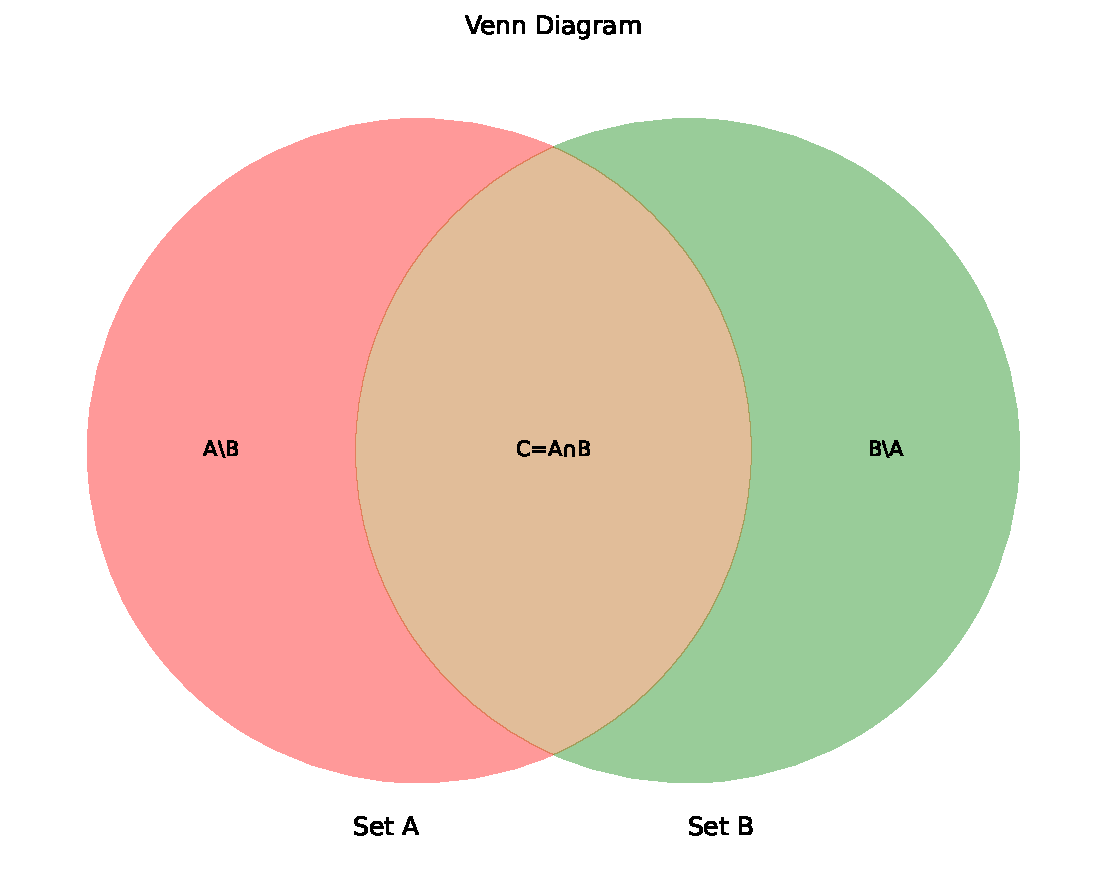
\includegraphics[keepaspectratio]{法律家のための統計数理1_files/figure-beamer/cell-2-output-1.pdf}}

\subsubsection{条件付き確率の定義}\label{sec-conditional-probability}

\begin{tcolorbox}[enhanced jigsaw, toprule=.15mm, leftrule=.75mm, titlerule=0mm, bottomtitle=1mm, title={定義(条件付き確率)}, arc=.35mm, toptitle=1mm, colbacktitle=quarto-callout-tip-color!10!white, coltitle=black, rightrule=.15mm, colback=white, opacityback=0, colframe=quarto-callout-tip-color-frame, opacitybacktitle=0.6, left=2mm, breakable, bottomrule=.15mm]

\(A,B\subset\Omega\) を事象とする. 事象 \(A\) が起こった場合の,事象
\(B\) の\textbf{条件付き確率}とは, \[
P(B|A):=\begin{cases}\frac{P(A\cap B)}{P(A)}&P(A)\ne0\;\text{のとき}\\0&P(A)=0\;\text{のとき}\end{cases}
\] という値を指す.\footnotemark{}

\end{tcolorbox}

\footnotetext{ここでは \(P(A)=0\) の場合は \(0\)
としたが,実際はどんな値でも良い.}

\subsubsection{式(1.7) p.7の証明}\label{ux5f0f1.7-p.7ux306eux8a3cux660e}

\begin{tcolorbox}[enhanced jigsaw, toprule=.15mm, leftrule=.75mm, titlerule=0mm, bottomtitle=1mm, title={式(1.7) p.7}, arc=.35mm, toptitle=1mm, colbacktitle=quarto-callout-tip-color!10!white, coltitle=black, rightrule=.15mm, colback=white, opacityback=0, colframe=quarto-callout-tip-color-frame, opacitybacktitle=0.6, left=2mm, breakable, bottomrule=.15mm]

\(A,B\subset\Omega\) を事象,\(P(A)>0\) とする. \[
P(A|B)+P(A^\complement|B)=1.
\]

\end{tcolorbox}

\begin{tcolorbox}[enhanced jigsaw, toprule=.15mm, leftrule=.75mm, titlerule=0mm, bottomtitle=1mm, title={証明}, arc=.35mm, toptitle=1mm, colbacktitle=quarto-callout-note-color!10!white, coltitle=black, rightrule=.15mm, colback=white, opacityback=0, colframe=quarto-callout-note-color-frame, opacitybacktitle=0.6, left=2mm, breakable, bottomrule=.15mm]

\[
\begin{align*}
&\quad P(A|B)+P(A^\complement|B)\\
&=\frac{P(A\cap B)}{P(B)}+\frac{P(A^\complement\cap B)}{P(B)}\\
&\overset{\text{[P2]}}{=}\frac{P((A\cap B)\sqcup (A^\complement\cap B))}{P(B)}\\
&=\frac{P(B)}{P(B)}=1.
\end{align*}
\]

\end{tcolorbox}

\subsection{【重要概念】統計的独立性}\label{sec-independent}

\subsubsection{定義}\label{ux5b9aux7fa9}

\begin{tcolorbox}[enhanced jigsaw, toprule=.15mm, leftrule=.75mm, titlerule=0mm, bottomtitle=1mm, title={定義(独立性)}, arc=.35mm, toptitle=1mm, colbacktitle=quarto-callout-tip-color!10!white, coltitle=black, rightrule=.15mm, colback=white, opacityback=0, colframe=quarto-callout-tip-color-frame, opacitybacktitle=0.6, left=2mm, breakable, bottomrule=.15mm]

2つの事象 \(A,B\subset\Omega\)
が\textbf{独立}であるとは,次を満たすことをいう: \[
P(A\cap B)=P(A)P(B).
\] このとき, \(A\perp\!\!\!\perp B\) と表す.

\end{tcolorbox}

この式は本書p.7
(1.8)式に一致している.これを「積の公式」として導出しているが,これは\textbf{実は独立性の定義とすべき性質である}.その意味するところを次節で解説する.

\subsubsection{条件付き確率による特徴付け}\label{ux6761ux4ef6ux4ed8ux304dux78baux7387ux306bux3088ux308bux7279ux5fb4ux4ed8ux3051}

Section~\ref{sec-2}
で「数学では何を定義として採用するかに任意性がある場合が多い」と言った.今回の「独立性」概念も,2つの同値な定義がある.しかし,「唯一やってはいけないことは定義が曖昧な状態で進むことである」とも言った.従って,どちらか片方を定義とし,「定義ともう一つの条件が同値である」という命題が生まれることになる.

この形の命題のことを(数学概念の)\textbf{特徴付け}
という.このことを解説する\href{https://ja.wikipedia.org/wiki/\%E7\%89\%B9\%E5\%BE\%B4\%E3\%81\%A5\%E3\%81\%91_(\%E6\%95\%B0\%E5\%AD\%A6)}{Wikipediaページ}もある.

\begin{tcolorbox}[enhanced jigsaw, toprule=.15mm, leftrule=.75mm, titlerule=0mm, bottomtitle=1mm, title={命題(独立性の特徴付け)}, arc=.35mm, toptitle=1mm, colbacktitle=quarto-callout-tip-color!10!white, coltitle=black, rightrule=.15mm, colback=white, opacityback=0, colframe=quarto-callout-tip-color-frame, opacitybacktitle=0.6, left=2mm, breakable, bottomrule=.15mm]

2つの事象 \(A,B\subset\Omega\) について,次の2条件は同値:

\begin{enumerate}
\def\labelenumi{\arabic{enumi}.}
\tightlist
\item
  \(A,B\) は独立である:\(A\perp\!\!\!\perp B\).
\item
  \(P(B|A)=P(B)\).
\end{enumerate}

\end{tcolorbox}

\begin{tcolorbox}[enhanced jigsaw, toprule=.15mm, leftrule=.75mm, titlerule=0mm, bottomtitle=1mm, title={証明}, arc=.35mm, toptitle=1mm, colbacktitle=quarto-callout-note-color!10!white, coltitle=black, rightrule=.15mm, colback=white, opacityback=0, colframe=quarto-callout-note-color-frame, opacitybacktitle=0.6, left=2mm, breakable, bottomrule=.15mm]

\(P[A]=0\) の場合,任意の \(B\) について(1),(2)はいずれも常に成り立つ.
あとは,\(P[A]\ne0\)の場合を考える. すると,条件付き確率の定義
\[P[A\cap B]=P[A]P[B|A]\]
を考えれば,この右辺が\(P[A]P[B]\)に等しいことと,\(P[B|A]=P[B]\)であることとは同値.

\end{tcolorbox}

本書では2.の性質の方を定義としているが, \(P(B|A)\) という量は,
\(P(A)=0\)
の場合に定義に任意性が残る.従って,1.の方が定義として明瞭ということになる.

さらに重要なことには,1.の方が一般個数の事象 \(A_1,\cdots,A_n\)
の場合に「独立性」の概念の拡張が可能であり,より本質的な定義だと思われる,ということが確率論の示唆である.実は,無限個の事象が独立であることも同様に定義する.

\begin{tcolorbox}[enhanced jigsaw, toprule=.15mm, leftrule=.75mm, titlerule=0mm, bottomtitle=1mm, title={定義(独立性)}, arc=.35mm, toptitle=1mm, colbacktitle=quarto-callout-tip-color!10!white, coltitle=black, rightrule=.15mm, colback=white, opacityback=0, colframe=quarto-callout-tip-color-frame, opacitybacktitle=0.6, left=2mm, breakable, bottomrule=.15mm]

集合族 \(\{A_\lambda\}_{\lambda\in\Lambda}\subset\mathcal{F}\)
が\textbf{独立}であるとは,任意の \(n\in\mathbb{N}\) 個の相異なる元
\(A_{\lambda_1},\cdots,A_{\lambda_n}\) に対して,
\[P[A_{\lambda_1}\cap\cdots\cap A_{\lambda_n}]=P[A_{\lambda_1}]\cdots P[A_{\lambda_n}]\]
が成り立つことをいう.

\end{tcolorbox}

\subsection{【余談】数学について}\label{ux4f59ux8ac7ux6570ux5b66ux306bux3064ux3044ux3066}

ここまでを読んだ読者の中で,「集合」「写像」の言葉に,定義が十分に提示されていないと感じたものがあるなら,あなたは極めて筋が良い.実は,これらの裏に全て厳密な定義があるのが数学であるが,今回は確率論に集中するために省いた.

実際,確率論をKolmogorovによる確率の公理的な定義
(\citeproc{ref-Kolmogorov1931}{Kolmogorov, 1931})
から始まる数学分野だとするならば,これはまだ100年の歴史もない,数学分野にしては極めて珍しい若い分野である.

確率論の確率が遅れた理由は,「確率」の概念がつかみどころのない日常に根ざした概念であり,抽象化が本質的に難しいこともあるだろうが,第一に「集合」「写像」といった概念が十分に数学者の間で理解が深まるのを待つ必要があったということがある.

現代の確率論では,「確率は測度の特別なものである」という態度をとっていることは本文中でも述べたが,この「測度」という概念の成立が,そもそもLebesgueによる積分論が確立される20世紀に入るのを待つ必要があった.

\phantomsection\label{refs}
\begin{CSLReferences}{1}{1}
\bibitem[\citeproctext]{ref-Ghosal-vanderVaart17-NonparametricBayes}
Ghosal, S., and van~der~Vaart, A. (2017). \emph{Fundamentals of
nonparametric bayesian inference},Vol. 44. Cambridge University Press.

\bibitem[\citeproctext]{ref-Kolmogorov1931}
Kolmogorov, A. (1931). Analytical methods in probability theory.
\emph{Über Die Analytischen Methoden in Der
Wahrscheinlichkeitsrechnung}, \emph{104}(1), 415--458.

\bibitem[\citeproctext]{ref-McElreath20-StatisticalRethinking}
McElreath, R. (2020). \emph{Statistical rethinking}. Chapman \& Hall.

\bibitem[\citeproctext]{ref-Rubin84-ABC}
Rubin, D. B. (1984). Bayesianly justifiable and relevant frequency
calculations for the applied statistician. \emph{The Annals of
Statistics}, \emph{12}(4), 1151--1172.

\bibitem[\citeproctext]{ref-ux5317ux5dddux654fux753749-ux7d71ux8a08ux5b66ux306eux8a8dux8b58}
北川敏男. (1949). \emph{統計学の認識}. 白揚社.

\bibitem[\citeproctext]{ref-ux5927ux585a2020}
大塚淳. (2020). \emph{\href{}{統計学を哲学する}}. 名古屋大学出版会.

\bibitem[\citeproctext]{ref-ux8349ux91ceux8015ux4e002016}
草野耕一. (2016).
\emph{\href{https://www.yuhikaku.co.jp/books/detail/9784641125889}{数理法務のすすめ}}.
有斐閣.

\end{CSLReferences}




\end{document}
